
\documentclass{jtetiproposalskripsi}

%-----------------------------------------------------------------
%Disini awal masukan untuk data proposal skripsi
%-----------------------------------------------------------------
\titleind{Merancang bangun aplikasi pengolahan administrasi yang efektif dan efisien serta informasi pemberitahuan BEM FT Universitas Muhammadiyah Jember}
\fullname{MERI APRILLIANTONO PUTRI}

\idnum{1200631045}

\approvaldate{14 Januari 2015}

\degree{Sarjana Komputer}

\yearsubmit{2015}

\program{Manajemen Informatika}

\headprogram{Bagus Setya Rintyarna, S.T, M.Kom}

%\dept{Manajemen Informatika dan Teknik Informatika}

\firstsupervisor{Triawan Adi Cahyanto, M.Kom}
\firstnip{12 03 719}

\secondsupervisor{Bagus Setya Rintyarna, S.T, M.Kom}
\secondnip{09 03 521}


%-----------------------------------------------------------------
%Disini akhir masukan untuk data proposal skripsi
%-----------------------------------------------------------------

\begin{document}

\cover

\approvalpage

%-----------------------------------------------------------------
%Disini akhir masukan untuk muka skripsi
%-----------------------------------------------------------------

%-----------------------------------------------------------------
%Disini awal masukan Intisari
%-----------------------------------------------------------------
\begin{abstractind}
Setiap orang membutuhkan komunikasi dengan orang lain dan mendapatkan informasi, baik secara langsung maupun melalui media.Dengan adanya rancangan BEM FT lebih mudah untuk pengelolahan administrasinya. Ikatan Mahasiswa Muhammadiyah khususnya di fakultas teknik Universitas Muhammadiyah Jember merupakan organisasi mahasiswa yang memiliki civitas cukup besar memerlukan sebuah wadah untuk bertemu dan berdiskusi dalam dunia maya tanpa terpengaruh oleh jarak dan waktu salah satunya BEM FT itu sendiri. Pada Tugas Akhir ini telah dibuat dengan aplikasi menggunakan bahasa pemrograman PHP, MySQL dan beberapa bahasa pemrograman pendukung diantaranya yaitu HTML.

\bigskip
\textbf{Keywords} : \emph{php, mysql}
\end{abstractind}
%-----------------------------------------------------------------
%Disini akhir masukan Intisari
%-----------------------------------------------------------------

\tableofcontents
\addcontentsline{toc}{chapter}{DAFTAR ISI}
\selectlanguage{bahasa}\clearpage\pagenumbering{arabic}\setcounter{page}{1}

%-----------------------------------------------------------------
%Disini awal masukan untuk Bab
%-----------------------------------------------------------------
\chapter{LATAR BELAKANG}

\section{Latar Belakang Masalah}

Teknologi dan informasi merupakan kesatuan sistem yang tidak dapat dipisahkan. Bagaimana tidak, hal ini sangat terlihat dari beberapa proses untuk mendapatkan informasi yang dapat diperoleh secara cepat, tepat, dan akurat, yang di dukung dengan kemajuan teknologi yang semakin canggih. Kemajuan teknologi ini membuat banyak organisasi menggunakan teknologi berbasis komputer untuk membantu mempermudah pekerjaan karena bersifat efektif dan efisien. 

Di lain sisi, suatu organisasi membutuhkan aplikasi-aplikasi yang dapat memudahkan dalam tertib administrasi dan komunikasi antar anggota organisasi.BEM FT merupakan gerakan mahasiswa atau wadah perjuangan untuk menghimpun, menggerakkan dan membina potensi mahasiswa guna meningkatkan peran dan tanggung jawabnya sebagai  mahasiswa aktif dalam organisasi. Selama ini pengolahan administrasi dalam organisasi masih dilakukan secara manual. Sering terjadinya salah komunikasi antar anggota dalam pemberitahuan rapat. Namun seiring dengan berjalannya waktu, perkembangan teknologi yang semakin meningkat akan membantu suatu organisasi untuk menyelesaikan administrasi dan masalah komunikasi dengan sebuah sistem secara efektif dan efisien.

Berawal dari masalah tersebut untuk membuat suatu organisasi bisa mencapai tujuan yang diinginkan melalui tertib administrasi organisasi dan terjalinnya komunikasi yang baik maka Aplikasi Kesekretariatan BEM FT inilah sebagai alternatif yang efektif untuk menghindari berbagai masalah yang dapat timbul dari penerapan sistem yang masih manual, misalnya lambatnya pencarian data atau informasi yang dibutuhkan, ataupun kesalahan dalam pencarian data sangat riskan terjadi. Permasalahan yang timbul tersebut dapat diminimalisir dengan penerapan sistem secara komputerisasi untuk pengolahan dan pengelolaan data, sehingga dapat membantu Sekretaris Umum Komisariat dalam melaksanakan proses administrasi.

\section{Perumusan Masalah}

Berdasarkan dari latar belakang di atas maka dapat dirumuskan masalah yaitu Bagaimana merancang dan membangun sebuah Aplikasi Kesekretariatan BEM FT Universitas Muhammadiyah Jember.

\section{Batasan Masalah}

Batasan masalah dalam perancangan dan pembuatan aplikasi ini, diantaranya adalah :
\begin{itemize}
\item[1.] Pembuatan Aplikasi Kesekretariatan dengan menggunakan Visual Basic dan Database menggunakan MySQL.
\item[2.] Aplikasi ini digunakan untuk organisasi BEM FT Universitas Muhammadiyah Jember.
\end{itemize}


\section{Tujuan Penelitian}
Tujuan penulis dalam penyusunan adalah merancang bangun aplikasi pengolahan administrasi yang efektif dan efisien serta informasi pemberitahuan BEM FT Universitas Muhammadiyah Jember.

\section{Manfaat Penelitian}
Manfaat dari dibuatnya program aplikasi ini yaitu :
\begin{itemize}
\item[1.] Memudahkan Struktural BEM FT dalam pengolahan administrasi organisasi serta pemberitahuan informasi rapat.
\item[2.] Sebagai alternatif yang efektif untuk pengolahan administrasi organisasi serta pemberitahuan informasi rapat. 
\item[3.] Menumbuhkan kesadaran kepada para Struktural BEM FT pentingnya tertib administrasi dan komunikasi antar anggota dalam suatu organisasi.
\end{itemize}

%-------------------------------------------------------------------------------
\chapter{Landasan Teori}
\section{Tentang Pembahasan BEM-FT Universitas Muhammadiyah Jember}

Ikatan Mahasiswa Muhammadiyah merupakan bagian dari AMM (Angkatan Muda Muhammadiyah) yang merupakan organisasi otonom di bawah Muhammadiyah. (Buhani. Najib : 2010)

Susunan organisasi dalam BEM-FT di buat secara berjenjang dari tingkat Mahasiswa Teknik.  Peraturan-peraturan dan keputusan-keputusan organisasi dalam lingkungannya masih di bawah naungan Dekan Fakultas Teknik karena di dalam organisasi BEM-FT itu sendri masih mahasiswa fakultas teknik dan setiap tahunnya selalu bergantian pengurus inilah Pembagian Tugas di BEM-FT:
\subsection{Ketua Umum :}
\begin{itemize}
\item[1.] Menjalankan fungsi kepemimpinan BEM FT Unmuh Jember.
\item[2.] Bertindak sebagai jiru bicara,monitoring,dan mempertahankan image BEM FT sebagai organisasi tertinggi di fakultas ternik.
\item[3.] Bertanggung jawab secara umum terhadap kelancaran kerja ke tataran coordinator disang.
\end{itemize}
\subsection{Wakil Ketua}
\begin{itemize}
\item[1.] Bertugas menggantikan tugas ketua umum ketika ketua tidak ada atau berhalangan hadir di dalam menjalankan fungsinya
\item[2.] Berkoordinasi secara intensif kepada ketua dan koordinasi bidang
\end{itemize}
\subsection{Sekretaris Umum}
\begin{itemize}
\item[1.] Mencatat hasil rapat.
\item[2.] Menginventaris segala barang di dalam BEM FT.
\item[3.] Berkoordinasi kepada ketua untuk setiap kegiatan.
\end{itemize}
\subsection{Bendahara Umum}
\begin{itemize}
\item[1.] Bertanggung jawab mengelola ,membuat laporankeuangan BEM FT
\item[2.] Bertanggungjawab terhadap kelancaran kinerja kebendarahaan
\end{itemize}
\subsection{PSDM}
\begin{itemize}
\item[1.] Bertanggungjawab dalam pembuatan event
\item[2.] Upgrading setiap HMJ
\end{itemize}
\subsection{HUMAS}
\begin{itemize}
\item[1.] Menjadi sumber informasi
\item[2.] Bertanggungjawab terhadap penyelenggaraan hubungan internal dan external
\end{itemize}
\subsection{KWN}
\begin{itemize}
\item[1.] Bertanggungjawab terhadap penyelenggaraan pengadaan sumber dana di BEM FT
\item[2.] Mendirikan dan mengembangkan badan usaha milik BEM FT
\end{itemize}
\subsection{PMT}
\begin{itemize}
\item[1.] Menampung semua keluhan mahasiswa
\item[2.] Menyampaikan semua catatan kedalam forum rapat.
\end{itemize}

\section{Struktur Organisasi IMM Tingkat Komisariat}
\begin{figure}[h]
\centering 
 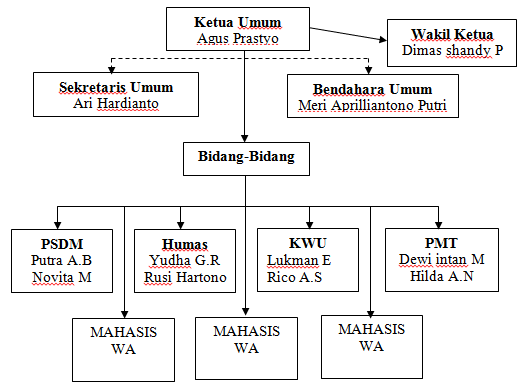
\includegraphics[width=0.7\textwidth]{gambar/1}  
 \caption{Struktural Organisasi}
\end{figure}
\section{Definisi Aplikasi}
Aplikasi adalah software yang bekerja pada suatu sistem operasi. Aplikasi akan menggunakan sistem operasi (OS) komputer dan aplikasi yang lainnya yang mendukung. Istilah ini mulai perlahan masuk ke dalam istilah Teknologi Informasi semenjak tahun 1993, yang biasanya juga disingkat dengan app. Secara historis, aplikasi adalah software yang dikembangkan oleh sebuah perusahaan. App Industri PC tampaknya menciptakan istilah ini untuk merefleksikan medan pertempuran persaingan yang baru, yang paralel dengan yang terjadi antar sistem operasi yang dimunculkan. (www.Google.com/Kamus Komputer dan Teknologi Informasi)
\section{Definisi Tentang Administrasi}
Istilah administrasi berasal dari bahasa latin yaitu “Ad” dan “ministrate” yang artinya pemberian jasa atau bantuan, yang dalam bahasa Inggris disebut “Administration” artinya “To Serve”, yaitu melayani dengan sebaik-baiknya.

Pengertian administrasi dapat dibedakan menjadi 2 pengertian yaitu :
\begin{itemize}
\item[1.] Administrasi dalam arti sempit. Menurut Soewarno Handayaningrat mengatakan“Administrasi secara sempit berasal dari kata Administratie (bahasa Belanda) yaitu meliputi kegiatan cata-mencatat, surat-menyurat, pembukuan ringan, keti-mengetik, agenda dan sebagainya yang bersifat teknis ketatausahaan”(1988:2).Dari definisi tersebut dapat disimpulkan administrasi dalam arti sempit merupakan kegiatan ketatausahaan yang mliputi kegiatan cata-mencatat, surat-menyurat, pembukuan dan pengarsipan surat serta hal-hal lainnya yang dimaksudkan untuk menyediakan informasi serta mempermudah memperoleh informasi kembali jika dibutuhkan.
\item[2.] Administrasi dalam arti luas. Menurut The Liang Gie mengatakan “Administrasi secara luas adalah serangkaian kegiatan yang dilakukan oleh sekelompok orang dalam suatu kerjasama untuk mencapai tujuan tertentu”(1980:9). Administrasi secara luas dapat disimpulkan pada dasarnya semua mengandung unsur pokok yang sama yaitu adanya kegiatan tertentu, adanya manusia yang melakukan kerjasama serta mencapai tujuan yang telah ditentukan sebelumnya.
\end{itemize}
\section{Tinjauan tentang Visual Basic}
Widodo (2002 : 86) menyatakan bahwa Visual Basic ialah bahasa pemograman event-driven yang berasal dari BASIC (Beginner All- Purpose Symbolic Intruction Code). Event-driven artinya program menunggu sampai adanya respon dari pemakai berupa kejadian tertentu, misalnya tombol diklik atau menu dipilih. Ketika event terdektesi, event yang berhubungan akan melakukan aksi sesuai dengan kode yang diberikan.

Konsep dasar pemograman Visual Basic 6.0 dari segi teknis hanya terdiri atas properti, metode dan event. Namun masalah masalah strategi pemograman seperti alokasi waktu saat mendesain software juga cukup penting sebagai landasan pengembangan software yang lebih baik. Kemampuan Microsoft Visual Basic 6.0 secara umum adalah menyediakan komponen-komponen yang memungkinkan untuk membuat program aplikasi yang sesuai dengan tampilan dan cara kerja Microsoft Windows. Guna membantu programmer dalam pembuatan program, Visual Basic menyediakan object-object yang sangat membantu.
\section{Tinjauan Alat-Alat Perancangan Sistem Informasi}
Untuk membangun sebuah sistem komputerisasi ataupun program aplikasi, terlebih dahulu harus menganalisa sistem yang sudah ada, yang nantinya akan diadakan perbaikan-perbaikan dan diberikan sebuah solusi yang tepat agar sistem tersebut dapat berjalan lebih afektif dan efisien. Tahap berikutnya Setelah analisa sistem selesai dilakukan adalah perancangan sistem. Adapun hal-hal yang perlu diperhatikan dalam sebuah perancangan sistem adalah mengenai rancangan sistem yang menggambarkan simbol-simbol aliran data ke dalam logika program.(Hartono,Jagiyanto.1990)
\section{Gambaran Sistem}
\subsection{Flowchart System}
Bagan alir sistem (system flowchart) merupakan bagan yang menunjukkan arus pekerjaan secara keseluruhan dari sistem. Bagan ini menjelaskan urut-urutan dari prosedur-prosedur yang ada di dalam sistem. Bagan alir sistem menunjukkan apa yang dikerjakan di sistem. Bagan alir sistem digambar dengan menggunakan simbol-simbol yang tampak sebagai berikut ini.(Hartono Jogiyanto.1990)
\newpage
\begin{center}
Tabel 2.1. Jadwal Penelitian.
\end{center}
\vspace{-0.5cm}
\begin{figure}[ht!]
  \centering
    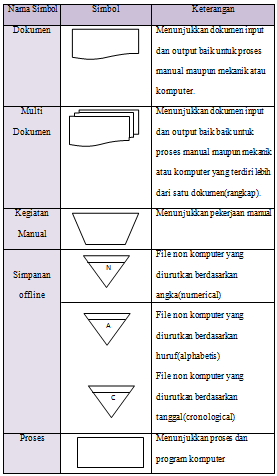
\includegraphics[width=12cm]{gambar/2}
\end{figure}
\begin{figure}[ht!]
  \centering
    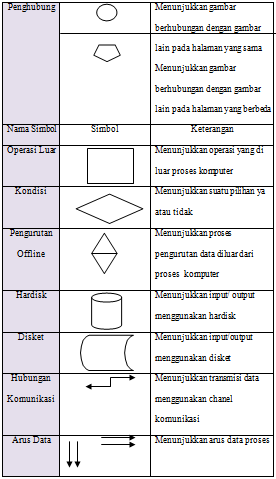
\includegraphics[width=12cm]{gambar/3}
\end{figure}
\subsection{Data Flow Diagram (DFD)}
DFD merupakan diagram yang mengunakan notasi-notasi atau simbol-simbol untuk mengambarkan sistem jaringan kerja antar fungsi-fungsi yang berhubungan satu sama lain dengan aliran dan penyimpanan data (Hartono,Jagiyanto.1990). Adapun yang digunakan dalam DFD adalah:
\subsubsection{Kesatuan Luar (External Entity)}
Kesatuan luar (entity) di lingkungan luar sistem yang dapat berupa orang,organisasi atau sistem lainnya yang berada di lingkungan luarnya yang akan memberikan input atau menerima output dari sistem. Suatu kesatuan luar dapat disimbolkan dengan suatu notasi persegi panjang atau suatu persegi panjang dengan sisi kiri dan atasnya berbentuk garis tebal.
\subsubsection{Aliran data}
Aliran data di DFD diberikan simbol suatu panah. Aliran data ini mengalir diantara process (process), simpanan data (data store) dan kesatuan luar (External entity). Aliran data ini menunjukkan arus dari data yang dapat berupa masukan untuk sistem atau hasil dari proses sistem.
\subsubsection{Proses}
Suatu process adalah kegiatan atau kerja yang dilakukan oleh orang, mesin atau komputer dari hasil suatu aliran datayang masuk ke dalam proses untuk dihasilkan aliran data yang akan keluar dari proses. Suatu proses dapat disimbolkan dengan notasi lingkaran atau dengan simbol empat persegi panjang dengan sudut-sudut tumpul.
\subsubsection{Penyimpan Data (Data Store)}
Penyimpan data (data store) merupakan penyimpan data yang dapat berupa:
\begin{itemize}
\item[1.] Suatu file atau basis data di sistem komputer.
\item[2.] Suatu arsip atau catatan manual.
\item[3.] Suatu kotak tempat data di meja seseorang.
\item[4.] Suatu tabel acuan manual.
\item[5.] Suatu agenda atau buku.
\end{itemize}

Simpanan data di DFD dapat disimbolkan dengan sepasang garis horizontal paralel yang tertutup di salah satu ujungnya atau tanpa ditutup (Hartono,Jagiyanto.2005). Adapun simbol yang digunakan Data Flow Diagram adalah sebagai berikut :
\begin{center}
Tabel 2.1. Simbol Flowshart
\end{center}
\vspace{-0.5cm}
\begin{figure}[ht!]
  \centering
    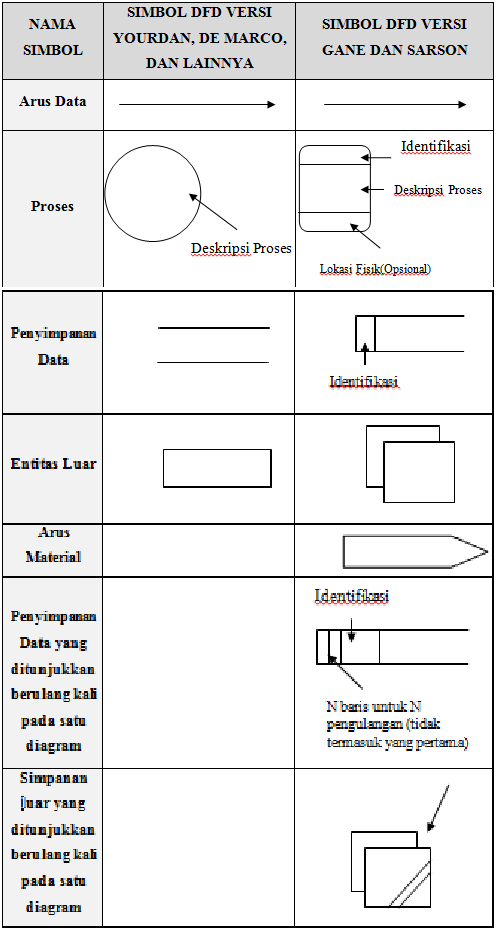
\includegraphics[width=10cm]{gambar/4}
\end{figure}

Dari tabel simbol DFD diatas penulis menggunakan simbol yang secara umum atau sering dipakai yaitu DFD versi Yourdan, De Marco, dan lain-lainnya.(Hartono,Jagiyanto.1990).
\section{Tinjauan tentang Database}

Database adalah kumpulan file-file yang mempunyai kaitan antara satu file dengan file yang lain sehingga membentuk satu bangunan data untuk menginformasikan satu perusahaan, instansi tersebut dalam batasan tertentu. Bila terdapat file yang tidak dapat dipadukan atau dihubungkan dengan file yang lainnya berarti file tersebut bukanlah kelompok dari satu database, akan membentuk satu database tersendiri. (Kristanto, 1994).
	
Basis data (database) merupakan kumpulan dari data yang saling berhubungan satu dengan yang lainnya, tersimpan di perangkat keras komputer dan digunakan perangkat lunak untuk memanipulasinya. Database merupakan salah satu komponen yang penting dalam sistem informasi, karena merupakan basis dalam menyediakan informasi bagi para pemakai. (Hartono,1999).

Basis data merupakan kumpulan dari data yang saling berhubungan satu dengan yang lainnya, di simpanan luar komputer dan menggunakan perangkat lunak tertentu untuk memanipulasinya. Database merupakan salah  satu komponen yang penting di sistem informasi, karena berfungsi sebagai  basis penyedia informasi bagi para pemakainya. Penerapan database dalam  sistem informasi disebut dengan database system. Sistem basis data (database system) ini adalah suatu sistem informasi yang mengintegrasikan kumpulan dari data yang saling berhubungan satu dengan lainnya dan membuatnya tersedia untuk beberapa aplikasi yang bermacam-macam di dalam  suatu organisasi. Tujuan dari desain database adalah untuk menentukan data-data yang dibutuhkan dalam sistem, sehingga informasi yang dihasilkan dapat terpenuhi dengan baik.


%-------------------------------------------------------------------------------
\chapter{METODOLOGI}

\section{Alat dan Bahan}

Dalam pelaksanaan dan penyusunan Laporan Tugas Akhir (TA) ini digunakan bahan dan alat sebagai berikut :
\subsection{Perangkat Keras}
Perangkat Keras (Hardware) yang digunakan dalam pembuatan perancangan aplikasi ini adalah satu unit komputer dingan spesifikasi sebagai berikut :
\begin{itemize}
\item[1.] Motherboard Intel PCChips P51G
\item[2.] Processor Intel(R) Core(TM) i3-2330 M 2.20 GHz
\item[3.] DDR3 2048MB RAM.
\end{itemize}
\subsection{Perangkat Lunak}
Perangkat Lunak (Software) yang digunakan dalam pembuatan Program Aplikasi ini antara lain :
\begin{itemize}
\item[1.] Operating System Microsoft Windows 8 pro 32-bit (6.2 , Build 9200)
\item[2.] Microsoft Office Visio 2007
\item[3.] Microsoft Visual Basic 6.0
\item[4.] MySQL
\end{itemize}
\section{Objek Penelitian}

Kegiatan Penelitian ini mengambil lokasi di Fakultas Teknik Gedung B Lantai 1 tepatnya di Sekretariat BEM-FT yang terletak di Fakultas Teknik Universitas Muhammadiyah Jember..

\section{Metode Penelitian}
\subsection{Studi Literatur}
Penelitian dilakukan menggunakan sumber referensi berupa buku  administrasi BEM-FT tahun 2008. Dan menggunakan wawancara terhadap pihak-pihak terkait.
\subsection{Pengumpulan Data}
Mencari  dan  mengumpulkan  data-data  yang  dibutuhkan  dan berkaitan dingan BEM-FT dan Pedoman Administrasi tahun 2008 beserta mahasiswa yang menjadi pengurus BEM-FT sendiri. 
\subsection{Observasi}
Melakukan wawancara terhadap sumber terkait untuk mengetahui tugas pokok dan fungsi bidang-bidang yang terkait sebagai arahan pembangunan Aplikasi Kesekretariatan yang diinginkan.
\begin{itemize}
\item[a.] Ketua Umum untuk mengetahui struktural organisasi dan apa yang menjadi tugas-tugasnya. Kendala-kendala dalam pencapaian tertib administrasi organisasi yang salah satunya adalah kesibukan kuliah di antara anggota BEM-FT.
\item[b.] Pimpinan komisariat untuk mengetahui pentingnya tertib administrasi dalam sebuah organisasi.
\end{itemize}
\subsection{Uji Coba}
Uji coba akan di lakukan pada bidang-bidang terkait seperti ketua umum, dan sekretaris.
\section{Perancangan System}
Analisis sistem dibutuhkan untuk melihat cara atau modil sistem yang ada, sehingga dapat dipakai seoptimal mungkin dan sesuai dingan tujuan yang ingin dicapai. Maka langkah yang ditempuh adalah merancang suatu sistem secara komputerisasi agar dapat digunakan seefisien mungkin.
\subsection{Flowchart System}
Secara garis besar alur sistem informasi yang di buat dapat digambarkan dingan flowchart sistem dibawah ini :
\begin{figure}[h]
\centering 
 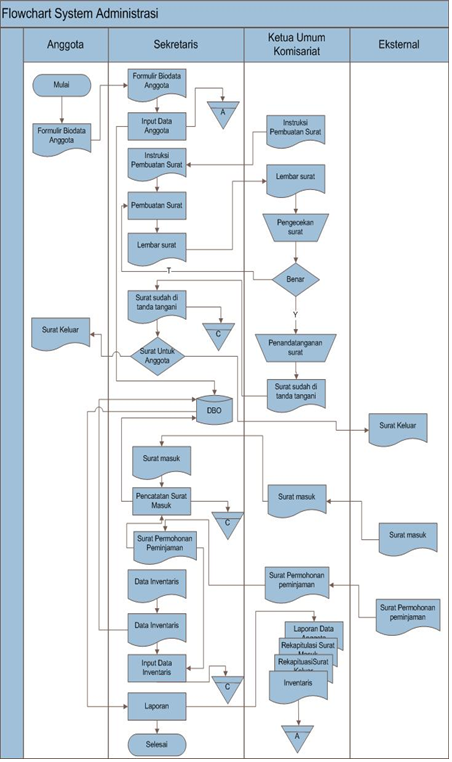
\includegraphics[width=0.65\textwidth]{gambar/5}  
 \caption{Flowchart System}
\end{figure}
\newpage
Keterangan Flowchart Sistem :
Mahasiswa yang tercatat sebagai anggota BEM-FT menyerahkan lembar biodata anggota yang telah diisi, sekretaris memeriksa dan memasukkan data-data anggota kedalam File Anggota. Kemudian lembar biodata anggota akan disimpan sebagai arsip.

Setelah proses memasukkan data-data anggota selesai, Sekretaris membuat surat sesuai dingan instruksi dari Ketua Umum yang kemudian di cetak dan diserahkan kepada Ketua Umum BEM-FT untuk dilakukan pengecekan dan penandatanganan surat. Apabila dalam pengecekan surat ada yang salah, maka sekretaris memperbarui dan membuat surat kembali. Apabila surat tersebut sudah benar maka akan di tanda tangani dan di kembalikan kepada sekretaris untuk di sebarkan. Apabila surat tersebut diberikan kepada anggota komisariat maka surat diserahkan kepada anggota komisariat. Apabila surat diserahkan kepada eksternal komisariat maka diberikan kepada komisariat-komisariat, maupun organisasi mahasiswa. Lembar surat yang sudah di tanda tangani akan disimpan sebagai arsip setelah digandakan.

Sekretaris mencatat dan memasukkan data-data surat masuk yag diperoleh dari komisariat-komisariat maupun organisasi mahasiswa lain secara manual dan lembaran surat akan disimpan sebagai arsip.
\newpage
\subsection{Perancangan Database}
\begin{itemize}
\item[a.] Tabel Anggota \\
\textit{Primary Key} = Id\_Anggota \\
\textit{Foreign Key} = -
\begin{center}
Tabel 3.1 Tabel Anggota
\end{center}
\vspace{-0.5cm}
\begin{figure}[ht!]
  \centering
    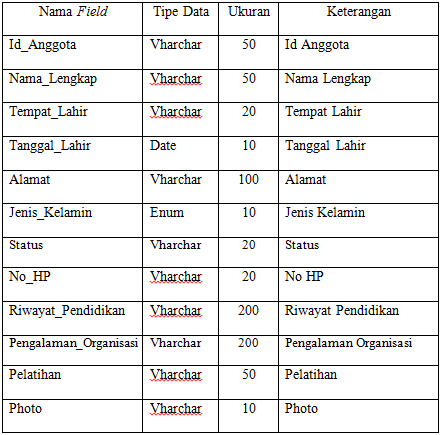
\includegraphics[width=15cm]{gambar/6}
\end{figure}
\newpage
\item[b.] Tabel Surat Keluar \\
\textit{Primary Key} = Kode\_Surat \\
\textit{Foreign Key} = Jenis\_Surat
\begin{center}
Tabel 3.2 Tabel Surat Keluar
\end{center}
\vspace{-0.5cm}
\begin{figure}[ht!]
  \centering
    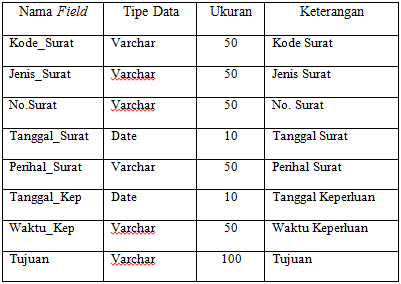
\includegraphics[width=15cm]{gambar/7}
\end{figure}
\newpage
\item[c.] Tabel Surat Masuk \\
\textit{Primary Key} = Kode\_Surat \\
\textit{Foreign Key} = Jenis\_Surat
\begin{center}
Tabel 3.3 Tabel Surat Masuk
\end{center}
\vspace{-0.5cm}
\begin{figure}[ht!]
  \centering
    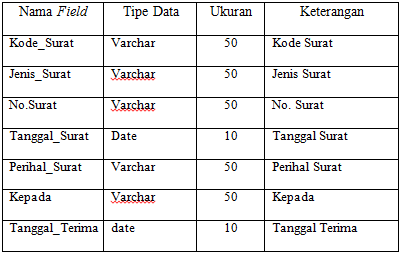
\includegraphics[width=15cm]{gambar/8}
\end{figure}

\end{itemize}

\end{document}